\documentclass[a4paper,11pt]{article}

\input ../include/preamble.tex

\usepackage{tikz}
\usetikzlibrary{automata,arrows,topaths,calc,positioning}

\begin{document}


\title{
    \textbf{Two hourglasses}\\
    \large{Programming II}
}
\author{Johan Montelius}
\date{Spring Term 2023}
\maketitle
\defaultpagestyle


\section*{Introduction}

This is a puzzle that you should solve using a method called {\em
  iterative deepening}. The procedure is to try to solve a puzzle in
the lest number of move by first trying to solve it with one move and
if that does not work, use two and of that does not work use three
etc. When you find a solution you know that this is the one with the
least number of moves.

This procedure is called iterative deepening since we iterate a try to
search for a solution deeper and deeper down in a search tree. It
sounds a bit inefficient to constantly start from the beginning but it
turns out that the overhead is not that big. The time it takes to find
a solution is not that bad compared to starting with the correct
depth directly.

\section*{The puzzle}

Assume that you have two hourglasses, one that can measure $7$ minutes
and one that can measure $4$ minutes. Your task is to come up with a
sequence of actions that will allow you to measure $13$ minutes. The
move that can do is of course to flip a hourglass over so that the
sand starts to fall into the lower chamber. You can of course flip any
of the glasses over whenever you want but since your task is to
measure time it only makes sense to flip it over when you know how
many minutes has passed.

\subsection*{the search three}

You can try to come up with a sequence right away but if you're not
Rain Man, it will probably take you some time. You will probably use a
pen and paper and start to write down sequences of move or what the
hourglasses look like after certain minutes. You probably realize that
we need a way to represent an hourglass so this will be your first job.

Once we have a suitable representation we need to define a search
tree; what does the tree look like, each node should be the state of
the two hourglasses but which {\em moves} are legal. When we search
the tree we should keep track of the depth but what is the depth and
what does a solution look like.

Let's represent an hourglass as for example [3,4] meaning that is is a
hourglass of seven minutes with three more minutes to go. We can then
display a search tree as follows:

\begin{figure}[h]
\center
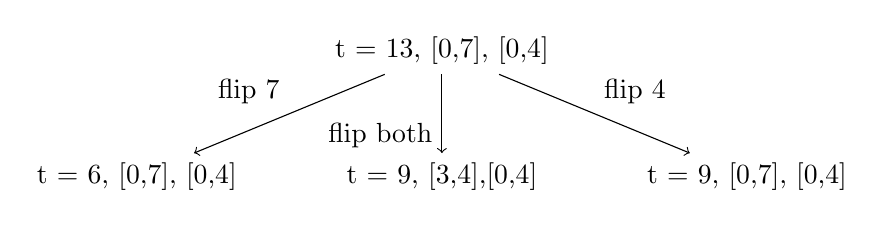
\begin{tikzpicture}[]
 \node[] (root) at (2,3) {t = 13, [0,7], [0,4]};

 \node[below left = of root] (a1) {t = 6, [0,7], [0,4]};
 \node[below = of root] (a2) {t = 9, [3,4],[0,4]};
 \node[below right = of root] (a3) {t = 9, [0,7], [0,4]};  
 \draw[->] (root) -- node[left, anchor = south east] {flip 7} (a1);
 \draw[->] (root) -- node[left, anchor = north east] {flip both} (a2);
 \draw[->] (root) -- node[right, anchor = south west] {flip 4} (a3);  
\end{tikzpicture}
\caption{The first level of the search three}
\end{figure}

This would be read as starting at time $0$ with the two hourglasses
standing on the table. We have three options: flip the first, both or
the second. If we flip the seven minutes glass only we can do nothing
but wait for seven minutes and again have the two hourglasses in front
of us. If we flip both we arrive at at state where we have three
minutes left in the seven minutes glass. The last option is to flip the second glass and wait for four minutes.

Note that we can not flip for example both glasses and wait for two
minutes and arrive to the situation: [5,2], [2,2]. We simply don't
know when two minutes has passed. We have to wait until one, or both,
glasses are down to zero and this is when do our next move.

If we expand the second branch we have the following tree:


\begin{figure}[h]
\center
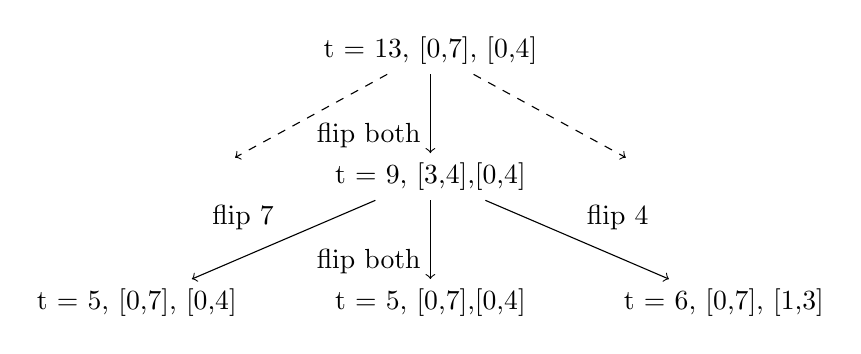
\begin{tikzpicture}[]
 \node[] (root) at (2,3) {t = 13, [0,7], [0,4]};

 \node[below left = of root] (a1) {}; 
 \node[below = of root] (a2) {t = 9, [3,4],[0,4]};
\node[below right = of root] (a3) {};  

 \draw[->, dashed] (root) -- (a1);
 \draw[->] (root) -- node[left, anchor = north east] {flip both} (a2);
 \draw[->, dashed] (root) -- (a3);

 \node[below left = of a2] (b1) {t = 5, [0,7], [0,4]};
 \node[below = of a2] (b2) {t = 5, [0,7],[0,4]};
 \node[below right = of a2] (b3) {t = 6, [0,7], [1,3]};  

 \draw[->] (a2) -- node[left, anchor = south east] {flip 7} (b1);
 \draw[->] (a2) -- node[left, anchor = north east] {flip both} (b2);
 \draw[->] (a2) -- node[right, anchor = south west] {flip 4} (b3);   
 
\end{tikzpicture}
\caption{Expanding the search three}
\end{figure}

If you start to draw the rest of this search tree you will find out
that it is rather big. It is of course not infinitely large since a
branch must stop if there is no time left (an time will be decreased
in each step). Since each node represents a state where one (or both)
hourglasses has A {\em solution} if found if we find a leaf with a time
of zero.

Since this puzzle comes in many flavors you should be able to solve
any specification of two hourglass of $x$ minutes and $y$ minutes and
measuring $z$ minutes (or determine that it is not possible). As you
will see the solution that you come up with will be able to do that so
don't worry.

\section*{check one solution}

The following is one possible way of step by step implement a program
that finds a solution to hour puzzle. You can follow this example or
come up with an alternative strategy.

Let's first settle for a representation of an hourglass. If it's an
hourglass standing on a table, we can represent it by the tuple {\tt
  \{:glass, 0, 7\}} meaning that this is an hourglass that can measure $7$
minutes. Once we flip it over the sand starts to trickle down, we need
to represent how much sand we have in the upper chamber and how much
we have in the lower chamber. An hourglass with flowing sand can then
be represented by the tuple {\tt \{:glass, 3, 4\}} meaning that four
minutes have passed and we have three more minutes to go.

We want to find a solution with as few {\em flips} as
possible. The iterative deepening method should therefore determine of
there is a solution with exactly $x$ flips before it tries to find a
solution with $x+1$ flips. We thus need a function that will determine
if there is a solution with exactly $z$ flips. Since we will do a lot
of flipping we might as well define a function that flips a hourglass.

\begin{minted}{elixir}
  def flip({:glas, t, n}) do {:glas, n, t} end  
\end{minted}

\subsection*{tick, tock}

We will search the tree using two functions: {\tt tick/4} and {\tt
  tock/4}. Both functions will take the two hourglasses, the number of
minutes that we should measure, {\tt k}, and exactly the number of
flips that we should do, {\t z}, as arguments.

The function {\tt tick/4} is used when we have flipped either of both
glasses and will move the time forward until either one of the
hourglasses has terminated.  As soon as one of the hourglasses
terminates we do have a choice and we then call {\tt tock/4} that will
explore the different options we have.

\begin{minted}{elixir}
  def tick({:glas, t1, n1}, {:glas, 0, n2}, k, z)  when t1 > 0 and t1 <= k do  
    tock({:glas, 0, n1+t1}, {:glas, 0, n2}, k-t1, z)
  end
   :
   :
\end{minted}

We of course have the reverse situation where the first glass is just
standing there and the second one is trickling sand. A third case is
if they are both trickling but the first one has less minutes to
go. The fourth case is the opposite and if there are no options (we would
run out of time) we return {\tt :no}.

So now we are ready to define {\tt tock/4}. We have two hourglasses, of
which at least one is down to zero. We now first check if we actually
have a solution and this is of course the case where both the minutes
and flips are down to zero. If they are we return {\tt :yes}.

\begin{minted}{elixir}
  def tock(_, _, 0, 0) do :yes end
\end{minted}

If we still have time to go but the number of flips that we should use
is down to zero there is no solution to be found.

\begin{minted}{elixir}
  def tock(_, _, _, 0) do :no end  
\end{minted}

In general we still have time to go and we have more flips to do so we
explore our options. The three options we have are: flip only the
first, only the second or both. Since it we are only looking for any
solution (not all or the best) we can try these options one by one. 

\begin{minted}{elixir}
  def tock(one, two, k, z) do
    case tock(flip(one), two, k, z-1) do 
       :no ->
         case .....  do
           :
         end
       :yes ->
          :yes     
    end
  end 
\end{minted}

Note that the flip-argument is decremented by one if we flip one glass
but by two if we flip both (you can of course choose to count flipping
both as one move).

If you implemented everything up to now you should be able to try the
following two calls:

\begin{minted}{elixir}
  Hour.tock({:glas, 0, 7}, {:glas, 0, 4}, 13, 5)
\end{minted}
and
\begin{minted}{elixir}
  Hour.tock({:glas, 0, 7}, {:glas, 0, 4}, 13, 6)
\end{minted}

If you done everything right you know that there is no solution using
exactly five flips but there is a solution using six flips. There
should be a solution with seven flips but not with eight. Is there one
for: 9, 10, 11, ...?

\section*{Iterative deepening}

The iterative deepening method is relative simple. You start by
searching for a solution using only zero flips (there are of course
none). When you know that there is no solution to be found you
increase the number of flips that you can use by one and try again. If
you find a solution you know that this is the "best" solution.


\begin{minted}{elixir}
  def solve() do
    solve({:glas, 0, 4}, {:glas, 0, 7}, 13)
  end
  
  def solve(one, two, k) do
    iterative(one, two, k, 0)
  end
  
  def iterative(one, two, k, z) do
    case ...    do
      :no ->
	...
      :yes ->
	{:found, z}
    end
  end
\end{minted}

If you get this right you should know that the best solution uses six
flips. You can call {\tt iterative/4} directly and find out that there
is another solution at seven, thirteen, ...

\begin{minted}{elixir}
  > Hour.iterative({:glas, 0, 7}, {:glas, 0, 4}, 13, 7)
   :

  > Hour.iterative({:glas, 0, 7}, {:glas, 0, 4}, 13, 8)
   :
\end{minted}

If you search for solutions with more flips you will eventually reach
a point where there are no more solutions. The way the iterative
deepening works right now you will then go into an endless search for
solutions by incrementing $z$. You might want to add a clause stating
that there is no point in searching for a solution with more than say
$2\times k$ flips. After all we can do at most two flips per minute.

 
\section*{The path}

So you know that there is a solution with $z$ flips but you still does
not know the order of these flips. We should therefore make a small
change to our program to generate a list of the moves we need to do.

The function {\tt tock/2} should return either {\tt :no} if no
solution can be found given the number of flips, or a list of flips
that we should do to find a solution. The flips could be encoded as
string for example "first", "second" or "both", or any way you choose
to do it.

Find the sequence of flips that will solve the puzzle in the least
number of flips.

\section*{The end}

So you have successfully solved the puzzle using a iterative deepening
strategy. What would the alternative be and how does your solution
compare? Have a you something that is easier to implement or does the
iterative strategy just add complexity to the code?

You will obviously do a lot of redundant computations since
you will have to explore the search space down to depth of $n-1$ all
for nothing if the solution is found at depth $n$. Estimate what the
extra work adds up; is it worth it?




  

\end{document}
